% !TEX root = Simulation.tex

\chapter{ALife - Text Chapter 8}

\section{ Problem 3 }
\textbf{ Choose one of the sample project of StarLogo and solve its exploration tasks (http://education.mit.edu/starlogo/projects.html). Write a brief report with the results obtained including any theoretical background knowledge that may eventually be necessary to perform the explorations. } \\
\newline
\textbf{Exploration questions:}\\
\textbf{Modify the program so that the creatures aggregate into a single large cluster more quickly.}\\
\textbf{How do the results change if there is more (or less) randomness in the creature's motion?}\\
\textbf{What "critical number" of creatures is needed for clusters to form? How does the critical number change if you change the evaporation or diffusion rate?}\\
\newline

By reducing the randomness, usually around 10 - 30, the creatures aggregated into a large cluster fairly quickly - a few minutes at most. Decreasing the rate of evaporation also decreased the aggregation time for the creatures since it would help 'catch' stray creatures. However, at the low random rates, such as in Figures ~\ref{mold1010}, ~\ref{mold2020} and ~\ref{mold3030} a creature or two would occasionally break free from the group and that would cause several others to also break free and form small clusters. This is well illustrated in Figure ~\ref{mold3030} where the middle images shows a fairly cohesive large cluster and the right image is after some groups broke free. 

Interestingly enough, with random values of 70, the creatures quickly formed small groups but were very slow to form two large groups, illustrated in Figure ~\ref{mold7070}. The two large groups would exchange members every now and then but never converged into a large group.

Around 500 - 600 hundred creatures while a pheromone evaporation of 2-4 was the 'critical number' for quick cluster formation. Too few creatures and they had a hard time finding each other. Too many creatures and there was too much pheromone deposited to form a big cluster. 

% 1010
\begin{figure}[tbh]
\begin{center}
	\begin{subfigure}[tbh]{0.30\textwidth}
	\begin{center}
	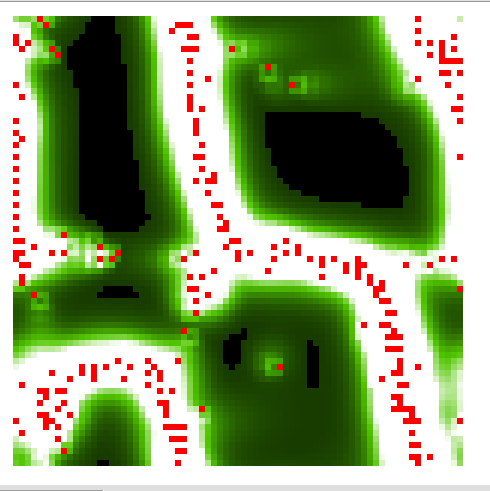
\includegraphics[width=\textwidth]{slimemold/mold10104-1.png}
	\end{center}
	\end{subfigure}
\hfill
	\begin{subfigure}[tbh]{0.30\textwidth}
	\begin{center}
	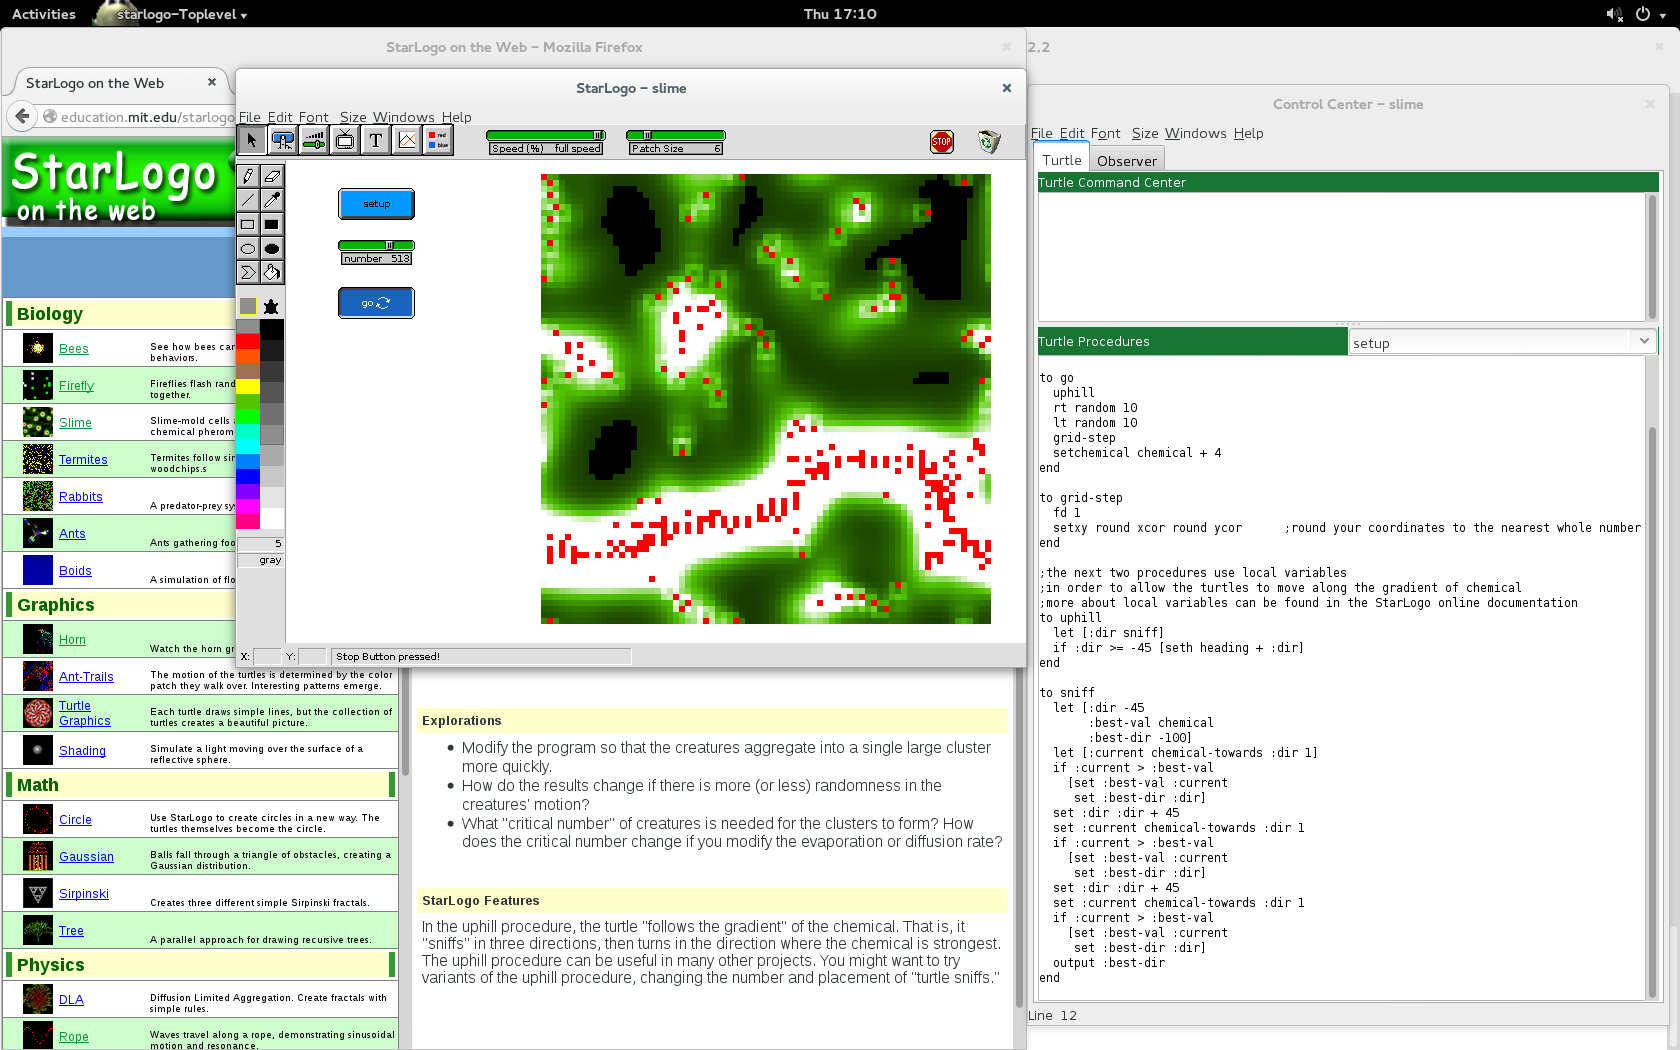
\includegraphics[width=\textwidth]{slimemold/mold10104-2.png}
	\end{center}
	\end{subfigure}
\hfill
	\begin{subfigure}[tbh]{0.30\textwidth}
	\begin{center}
	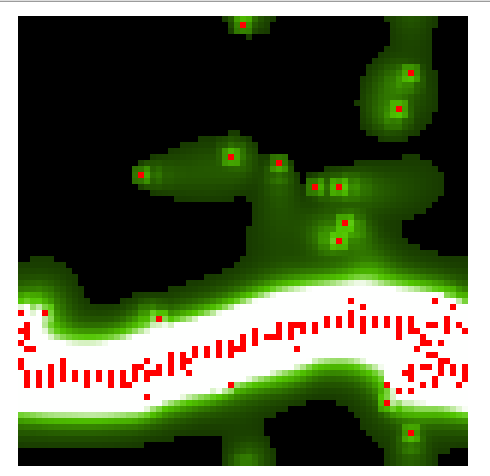
\includegraphics[width=\textwidth]{slimemold/mold10104-3.png}
	\end{center}
	\end{subfigure}
\caption{ Slime Mold with $x=10$ and $y=10$}
\end{center}
\end{figure} \label{mold1010}

%2020
\begin{figure}[tbh]
\begin{center}
	\begin{subfigure}[tbh]{0.30\textwidth}
	\begin{center}
	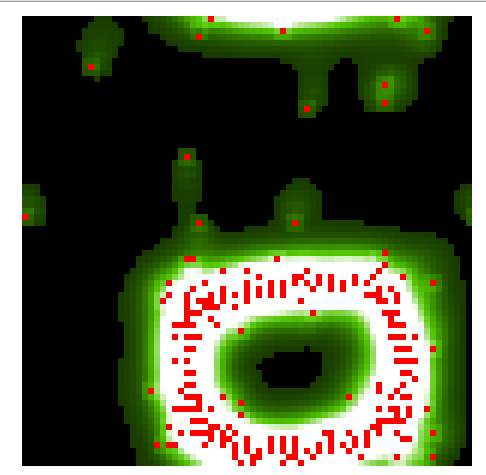
\includegraphics[width=\textwidth]{slimemold/mold20202-1.png}
	\end{center}
	\end{subfigure}
\hfill
	\begin{subfigure}[tbh]{0.30\textwidth}
	\begin{center}
	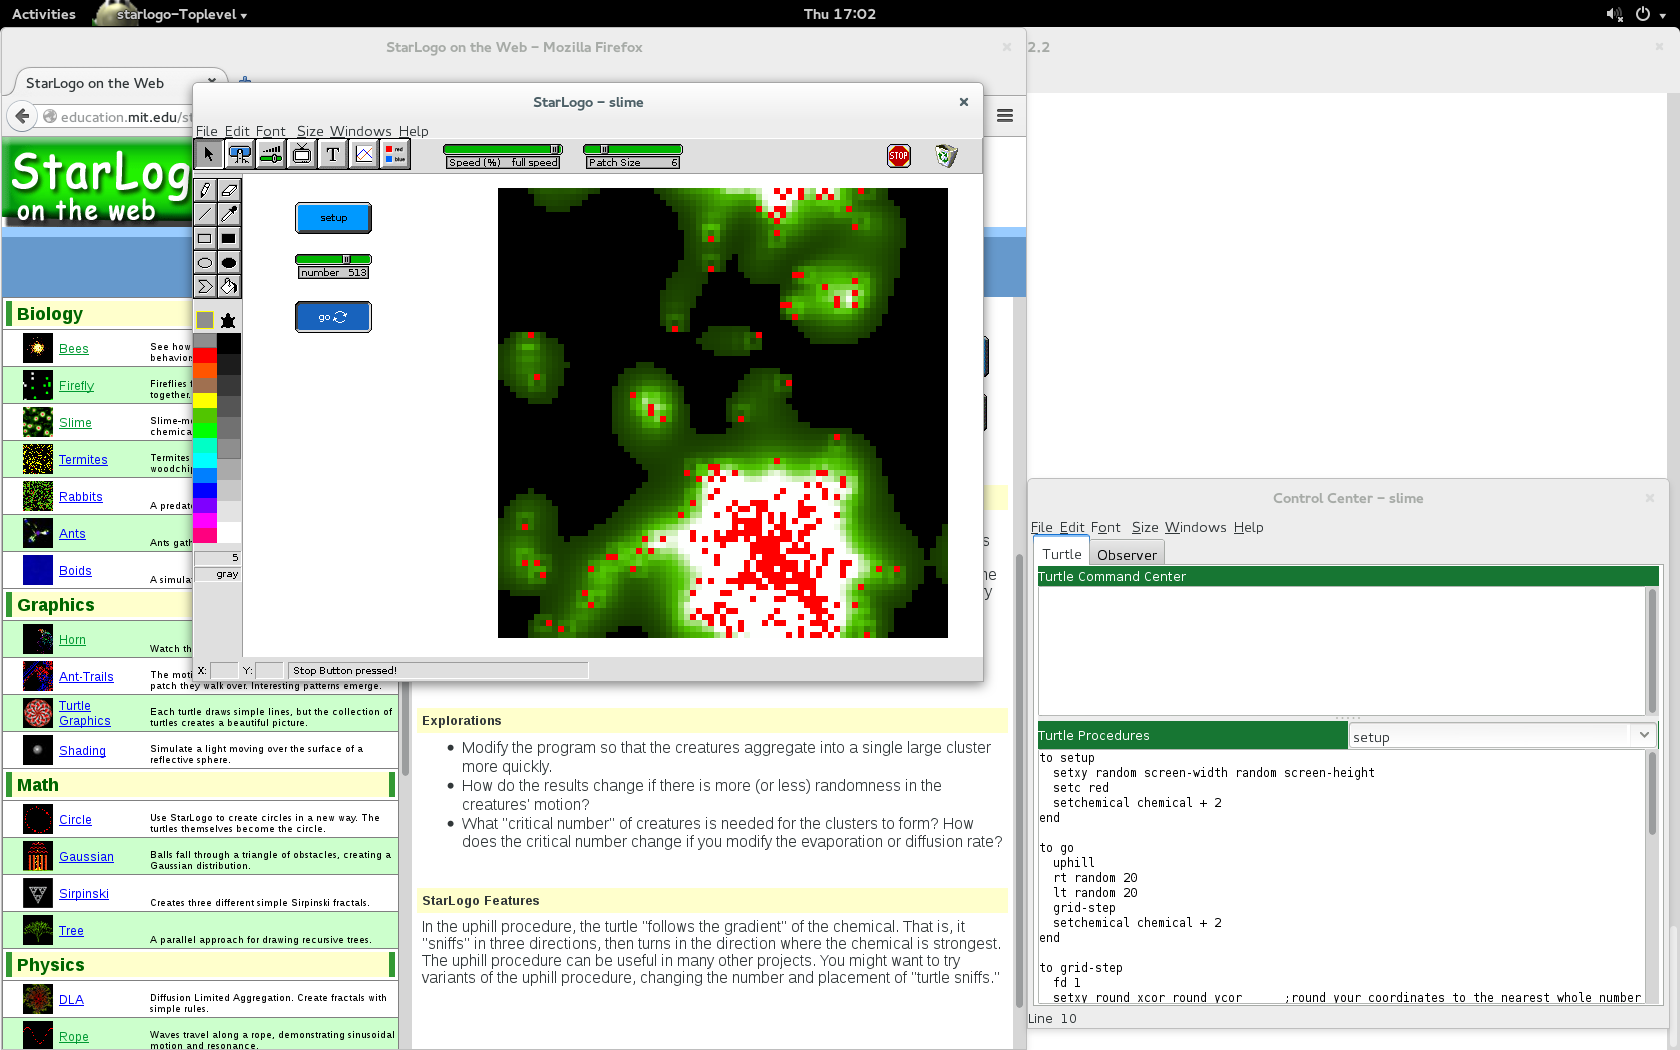
\includegraphics[width=\textwidth]{slimemold/mold20202-2.png}
	\end{center}
	\end{subfigure}
\hfill
	\begin{subfigure}[tbh]{0.30\textwidth}
	\begin{center}
	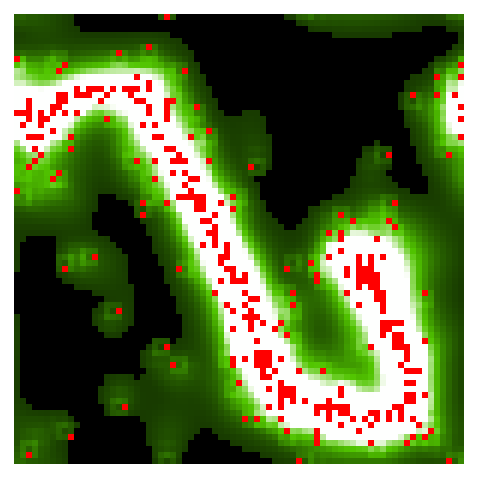
\includegraphics[width=\textwidth]{slimemold/mold20202-3.png}
	\end{center}
	\end{subfigure}
\caption{ Slime Mold with $x=20$ and $y=20$}
\end{center}
\end{figure} \label{mold2020}

%3030
\begin{figure}[tbh]
\begin{center}
	\begin{subfigure}[tbh]{0.30\textwidth}
	\begin{center}
	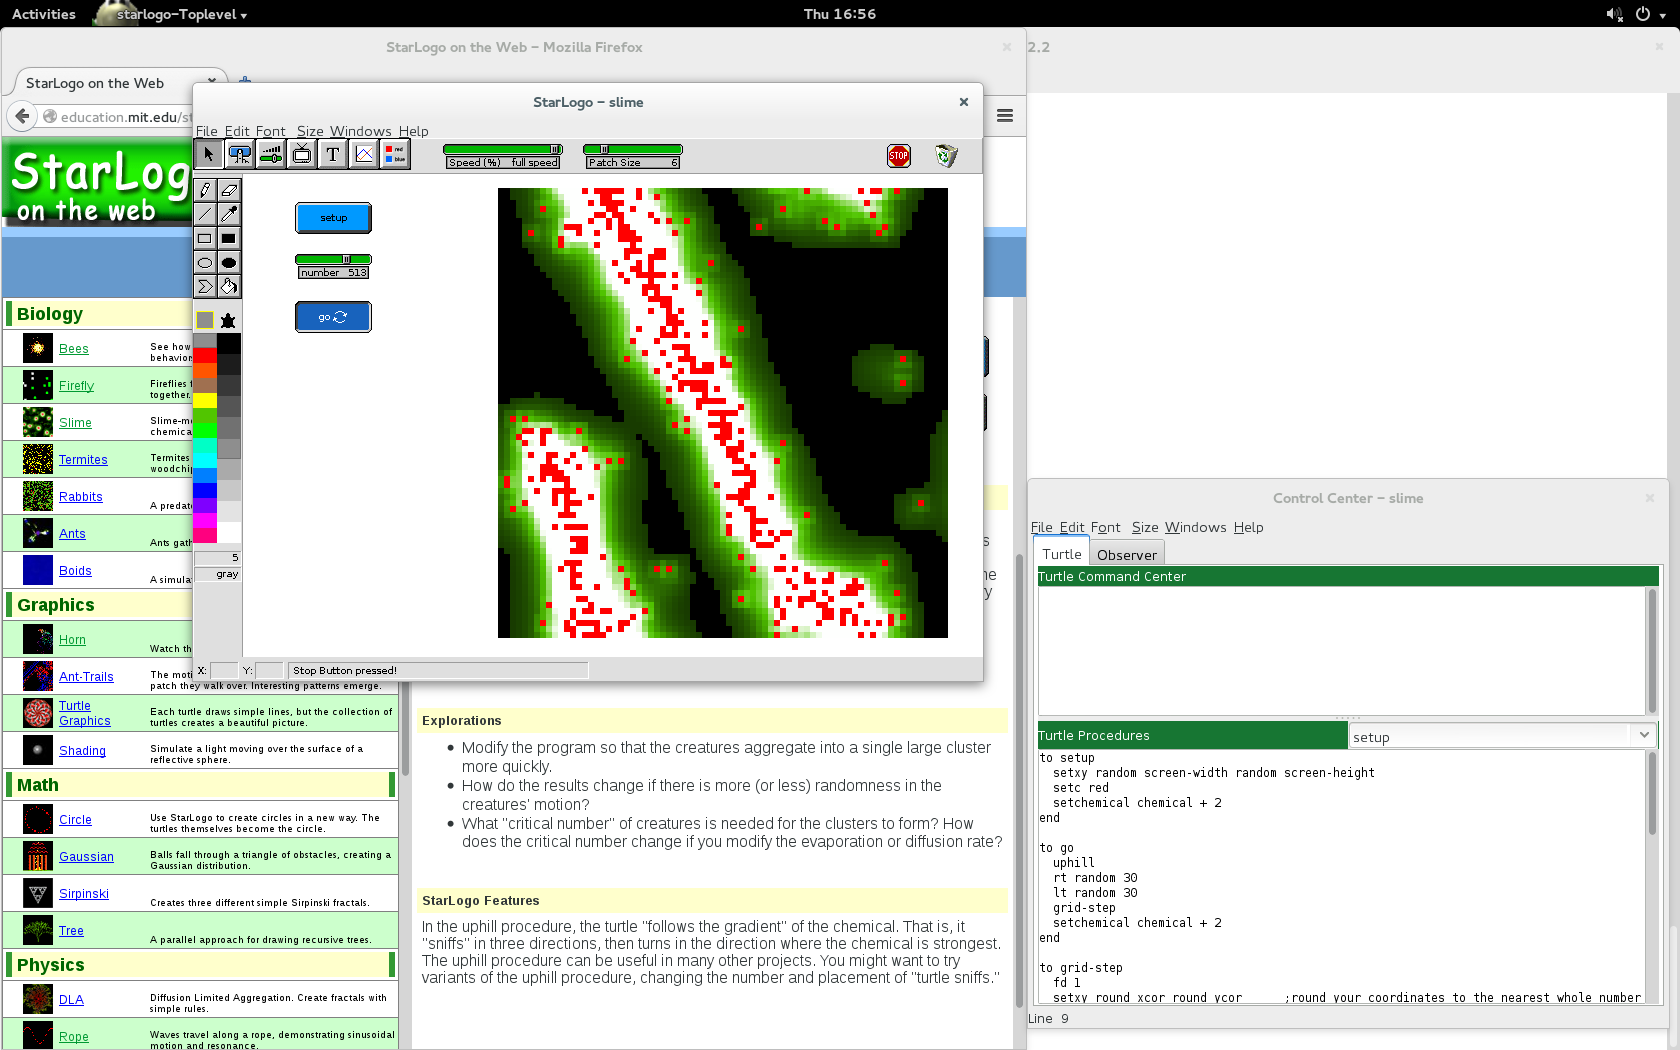
\includegraphics[width=\textwidth]{slimemold/mold30302-1.png}
	\end{center}
	\end{subfigure}
\hfill
	\begin{subfigure}[tbh]{0.30\textwidth}
	\begin{center}
	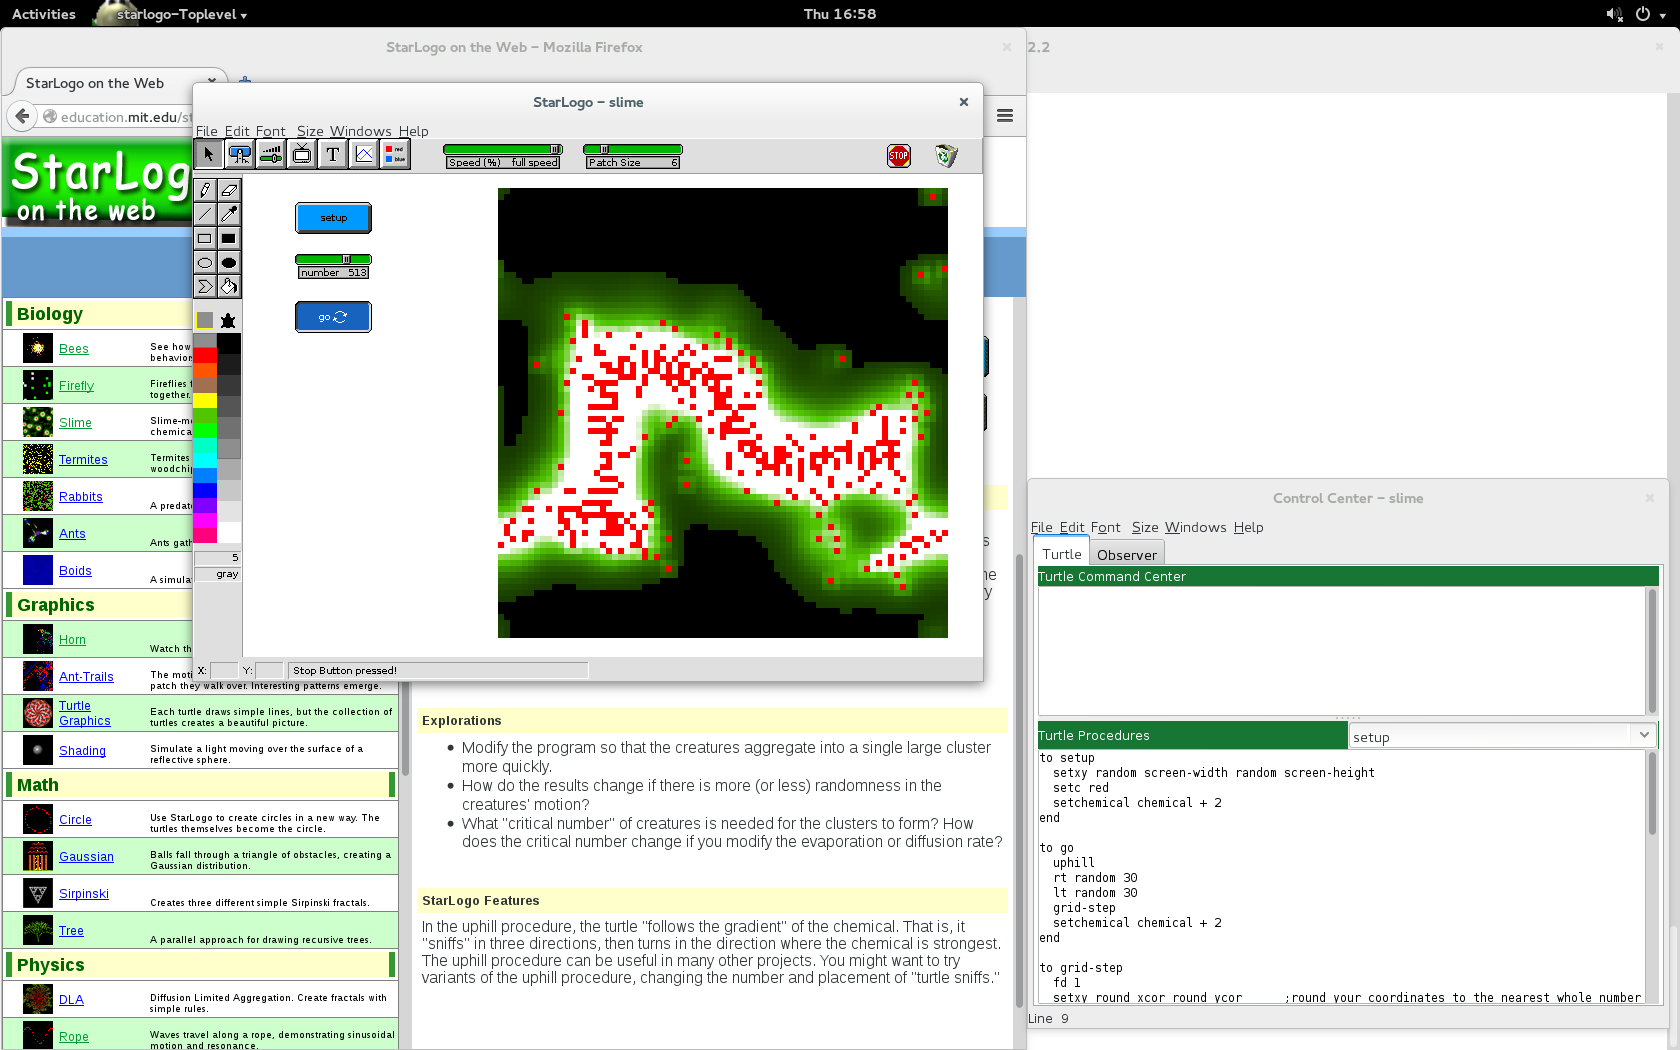
\includegraphics[width=\textwidth]{slimemold/mold30302-2.png}
	\end{center}
	\end{subfigure}
\hfill
	\begin{subfigure}[tbh]{0.30\textwidth}
	\begin{center}
	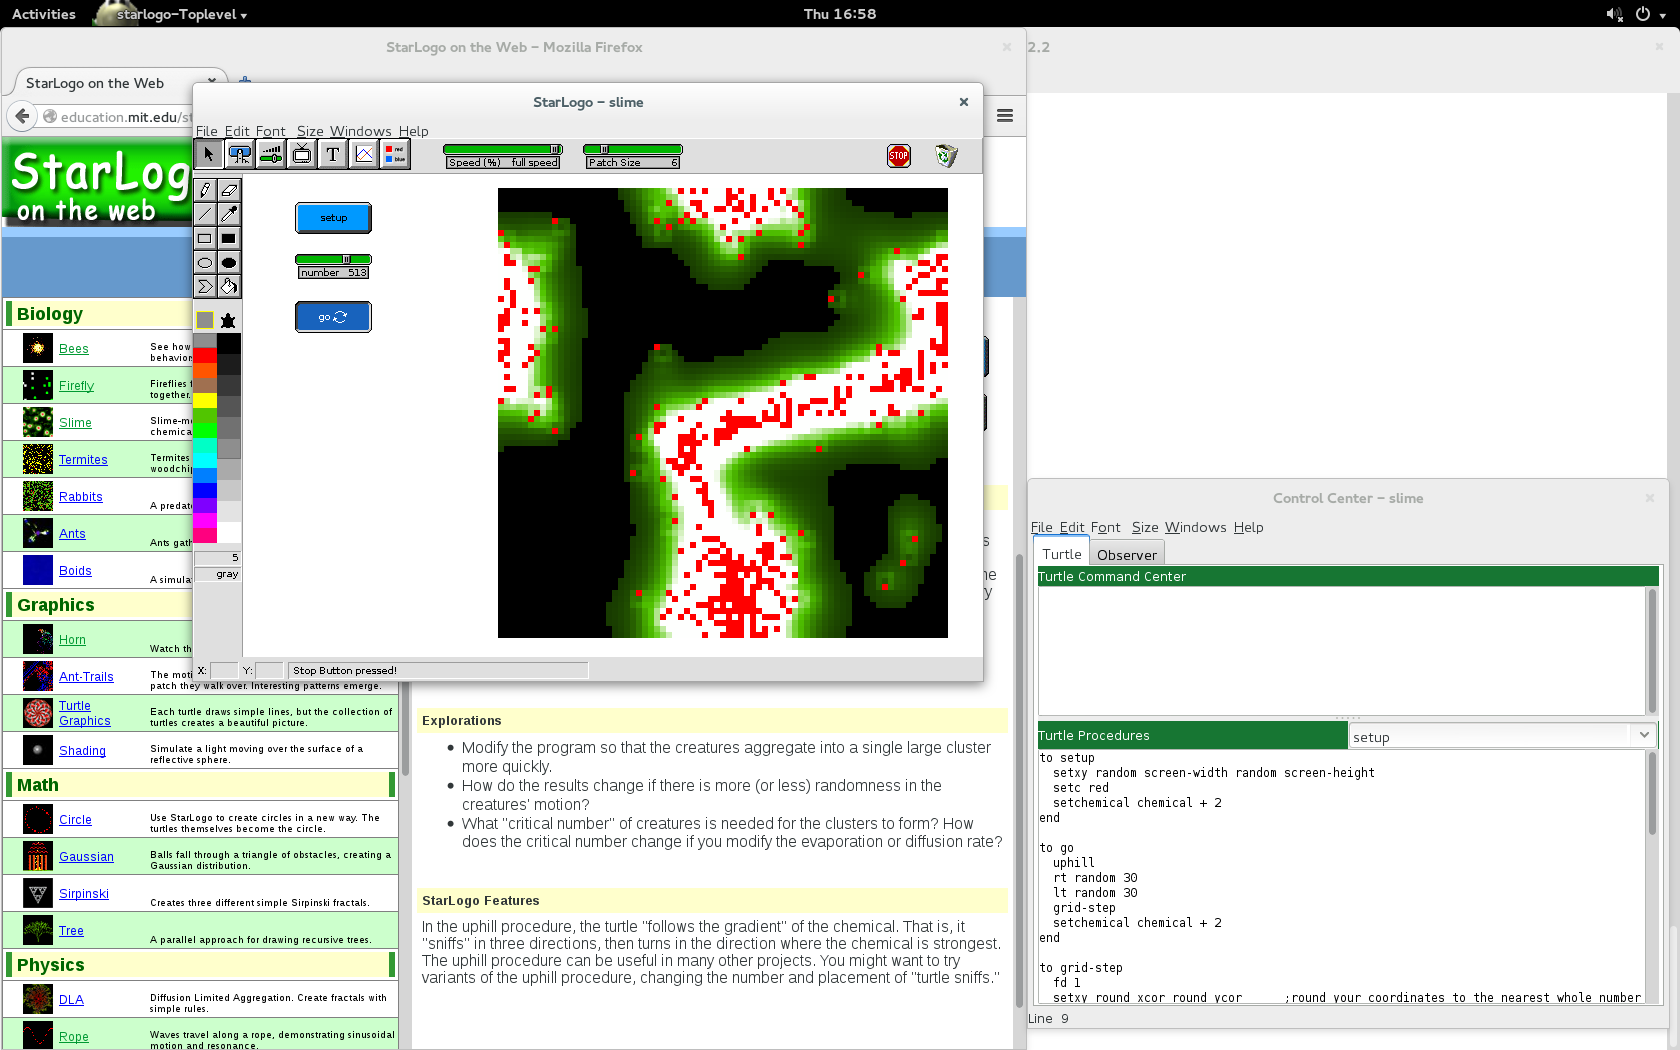
\includegraphics[width=\textwidth]{slimemold/mold30302-3diverge.png}
	\end{center}
	\end{subfigure}
\caption{ Slime Mold with $x=30$ and $y=30$}
\end{center}
\end{figure} \label{mold3030}

%7070

\begin{figure}[tbh]
\begin{center}
	\begin{subfigure}[tbh]{0.40\textwidth}
	\begin{center}
	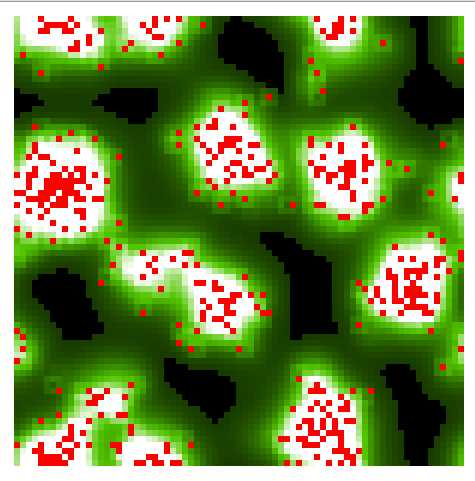
\includegraphics[width=\textwidth]{slimemold/mold70702-1.png}
	\end{center}
	\end{subfigure}
\hfill
	\begin{subfigure}[tbh]{0.40\textwidth}
	\begin{center}
	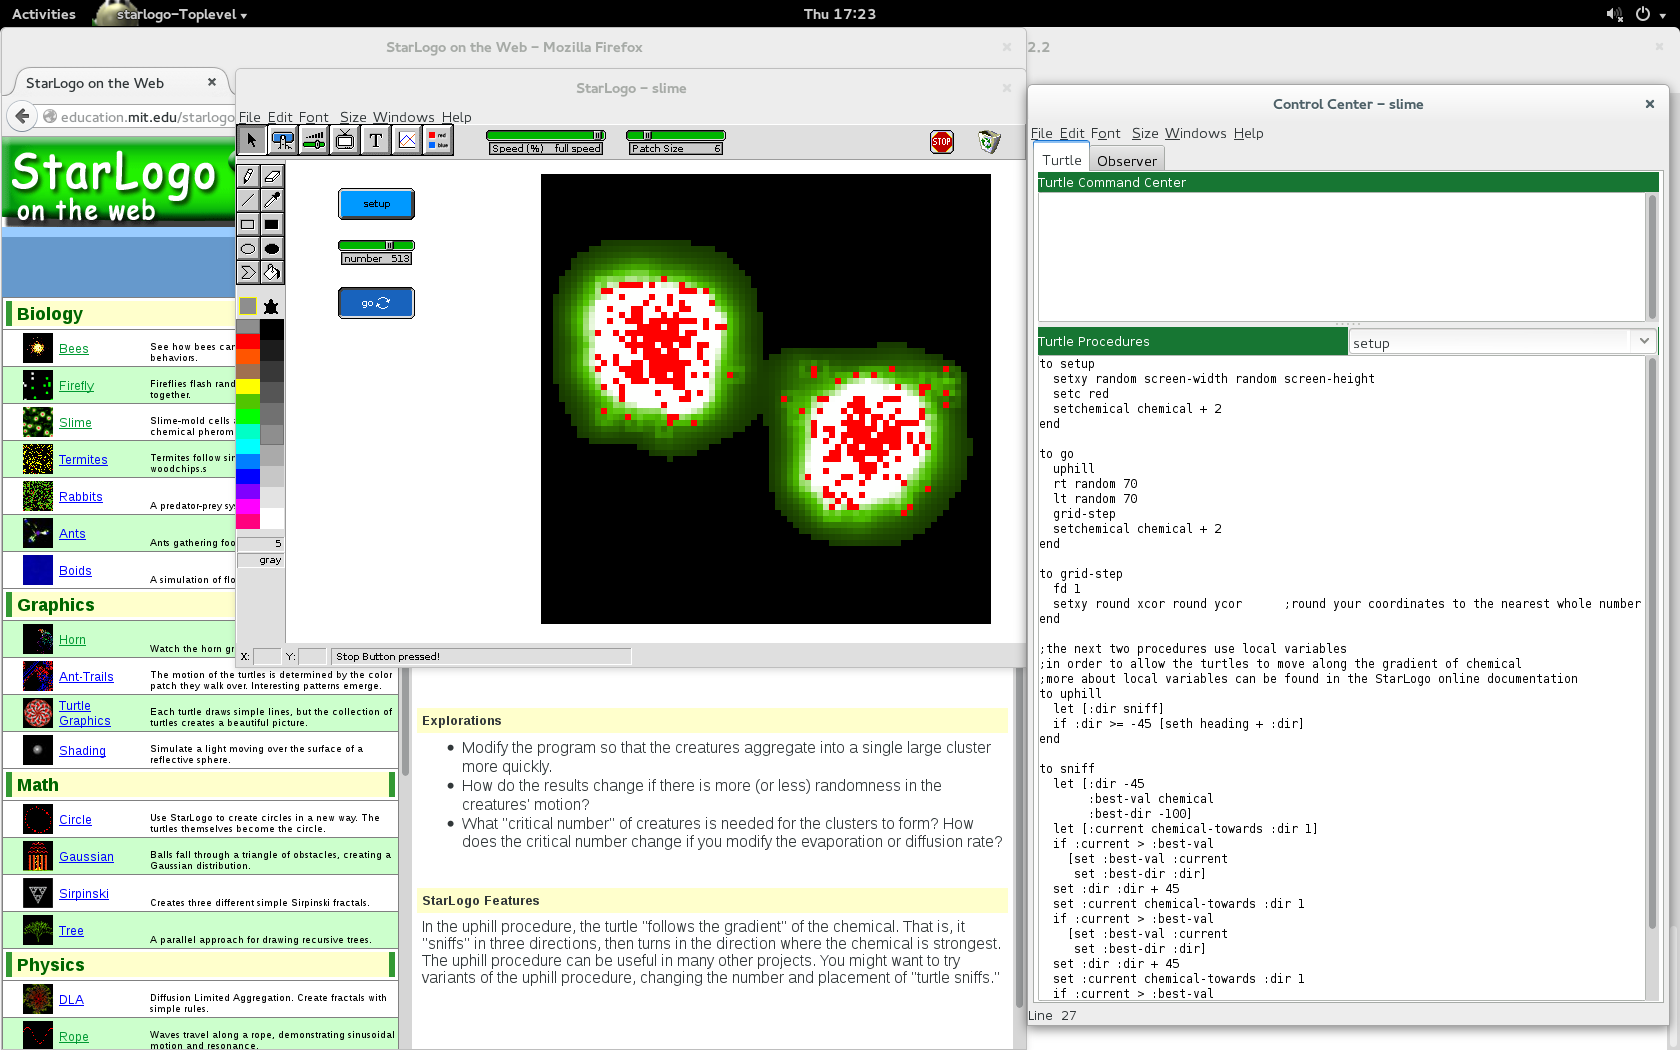
\includegraphics[width=\textwidth]{slimemold/mold70702-2.png}
	\end{center}
	\end{subfigure}
\caption{ Slime Mold with $x=70$ and $y=70$}
\end{center}
\end{figure} \label{mold7070}

\section{ Problem 4 }
\textbf{ Implement a bi-dimensional CA following the rules of ``The Game of Life.'' }\\
\newline
John Conway proposed a solitaire game called 'Life', currently known as 'The Game of Life'. He wanted to create a set of transition rules that were simple to write but also difficult to predict the outcome or overall behavior of the CA. The game had to meet the following criteria:

\begin{enumerate}
	\item There should not be any initial pattern for which there is a simple proof that the population can grow without limit.
	\item There should be initial patterns that apparently do grow without limit. Not all initial states should immediately yield trivial final states.
	\item There should be simple initial patterns that grow and change for a considerable period of time before coming to an end in three possible ways: fading away completely, settling into a stable configuration that remains unchanged thereafter, or entering an oscillating phase in which they repeat an endless cycle of two or more periods.
	\dots
\end{enumerate}

The rule set that Conway came up with is simple and uses the Moore neighborhood:
\begin{itemize}
    \item Birth: a previously dead cell comes alive if three neighbors are alive.
    \item Death: isolated living cells with no more than one live neighbor die; those with more than three neighbors die of overcrowding.
    \item Survival: living cells with two or three live neighbors survive.
	\dots
\end{itemize}

Using the above rule set and bi-directional grid, all of the criteria that Conway required appeared through running the Game of Life. There were oscillating phases and stable configurations that remained unchanged. A lot of the patterns died out or within a few generations turned into an stable configuration.

\begin{figure}[tbh]
\begin{center}
    \begin{subfigure}[tbh]{0.475\textwidth}
    \begin{center}
    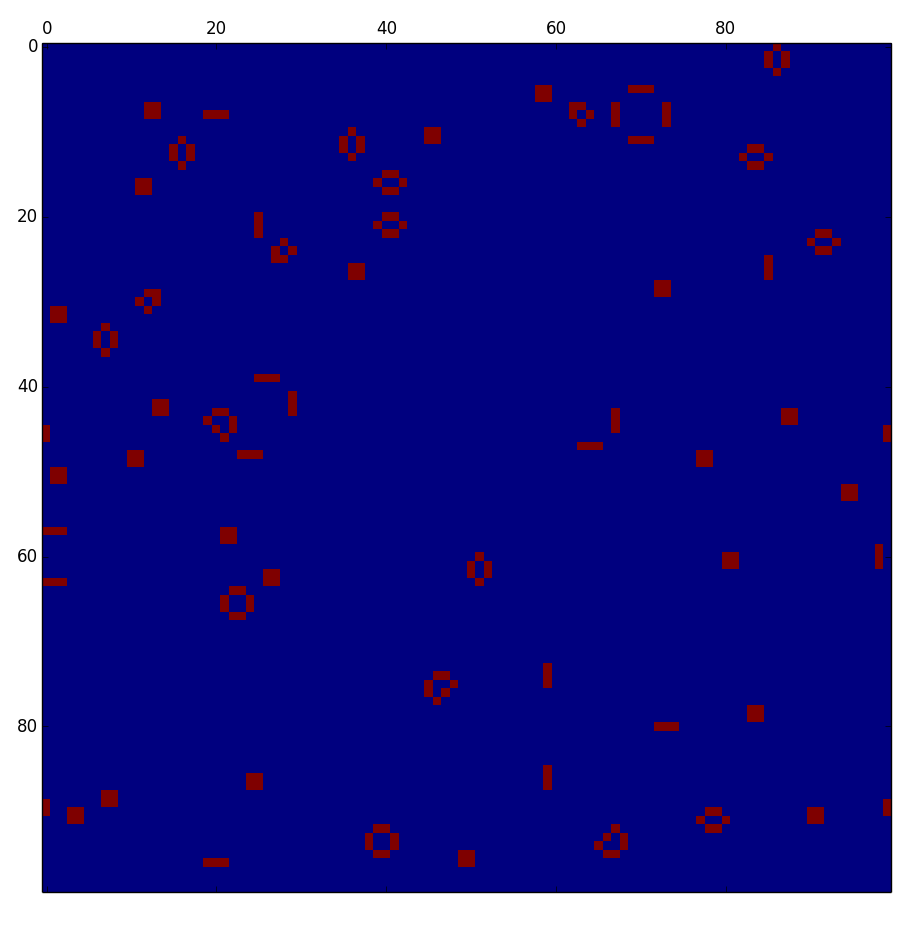
\includegraphics[width=\textwidth]{conway/game1.png}
    \caption{ Stabilized Game of Life with few oscillating phases }
    \end{center}
    \end{subfigure}
\hfill
    \begin{subfigure}[tbh]{0.475\textwidth}
    \begin{center}
    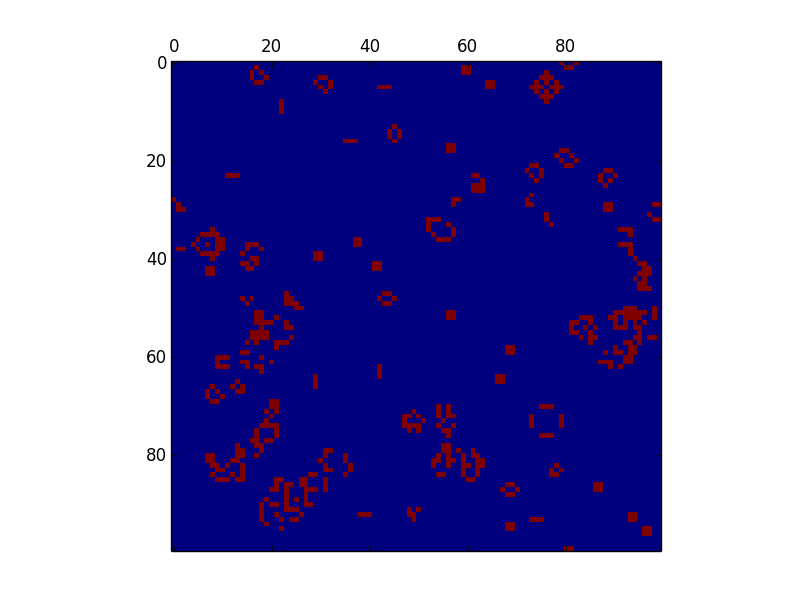
\includegraphics[width=\textwidth]{conway/game4.png}
    \caption{ Criteria 2 }
    \end{center}
    \end{subfigure}
\hfill
    \begin{subfigure}[tbh]{0.475\textwidth}
    \begin{center}
    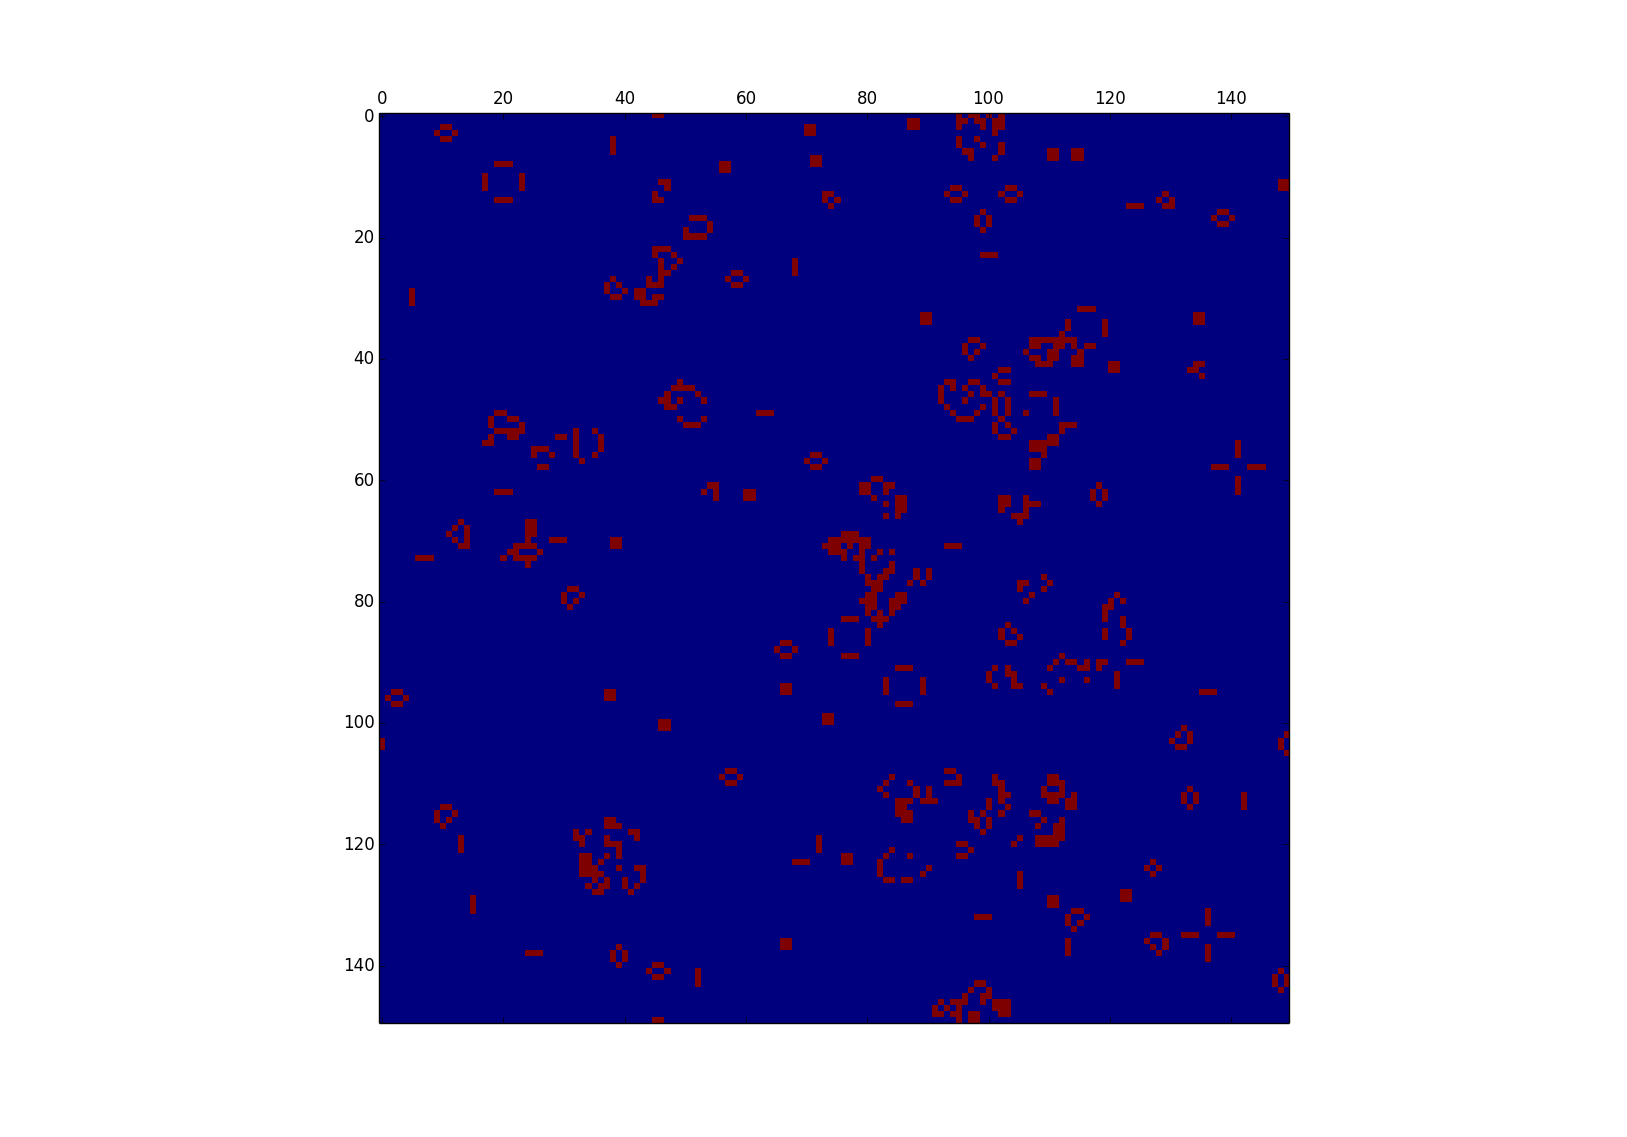
\includegraphics[width=\textwidth]{conway/game7.png}
    \caption{ Game in Progress }
    \end{center}
    \end{subfigure}
\hfill
    \begin{subfigure}[tbh]{0.475\textwidth}
    \begin{center}
    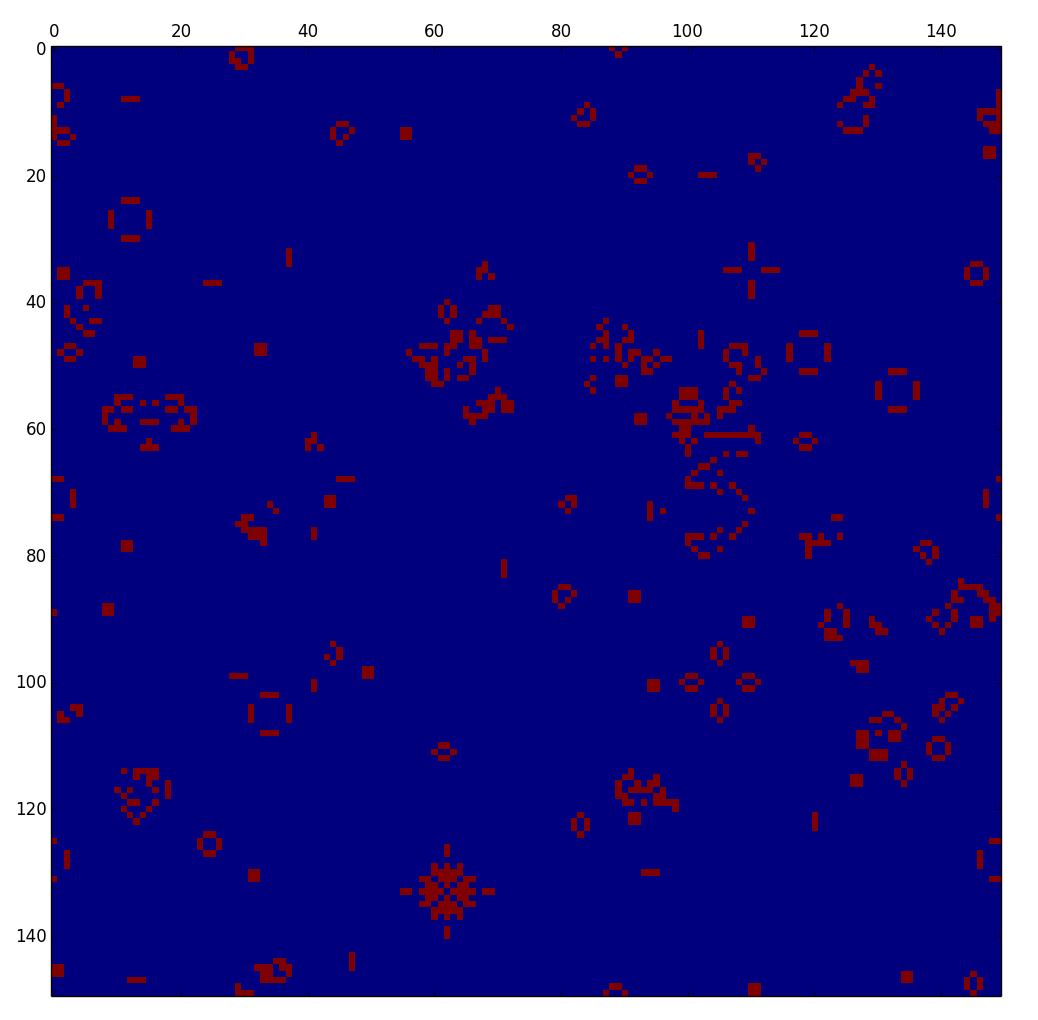
\includegraphics[width=\textwidth]{conway/game6.png}
    \caption{ Criteria 3 }
    \end{center}
    \end{subfigure}
\hfill
\end{center}
\caption{Plots of Various Games \label{conway} }
\end{figure}
